\section{Computational Methods}

Equilibrium MD simulations of a symmetric binary--mixture of two immiscible fluids (A and B) were used to measure the stresses acting on the fluid at two different temperatures and infer the Marangoni force using Eqn. \ref{FinDiff}.
Two key arrangements of such a mixture were studied, a symmetrical binary–mixture under three--dimensional periodic boundary conditions and a binary--mixture periodic in two--dimensions but held within two walls in the third-dimension, as shown in Fig. \ref{SetUp}.
All molecular dynamics simulations were executed using the LAMMPS (Large Atomic and Molecular Massively Parallel Simulator) package.\cite{LAMMPS}  

\begin{figure}[h]
        \includegraphics[scale=0.25]{AABB.png}
        \includegraphics[scale=0.25]{AABB_piston.png}
\caption{The system arrangements for a symmetric binary--mixture of two immiscible fluids under three-dimensional periodic boundary conditions (left) and a binary--mixture periodic in two--dimensions held within two walls (right) are shown. 
In the case of the three--dimensional boundary conditions, pressure must be controlled use a Nos\'{e}--Hoover barostat whilst for the fluid confined between two walls, these walls may be used as a piston to control the fluid pressure.}
\label{SetUp}
\end{figure}

\subsection{Interaction Model}\label{InteractionModel}
The fluids were modelled using spherical particles and their interaction was controlled using a pair--wuse truncated Lennard--Jones potential:
\begin{equation}
V \left( \mathbf{r}^{\mathrm{N}} \right) = \frac{1}{2} \sum_{i\neq j} \phi \left( r_{ij} \right)
\end{equation}
where
\begin{align}
\label{LJ}
\phi \left( r_{ij} \right) &= 4 \epsilon_{ij} \left( \left( \frac{\sigma_{ij}}{r_{ij}}\right)^{12} - \left( \frac{\sigma_{ij}}{r_{ij}}\right)^{6} \right)\ \mathrm{for}\ r < r_{c}\\
\phi \left( r_{ij} \right) &= 0\ \mathrm{otherwise}.
\end{align}
This potential involves an attractive $ri_{ij}^{-6}$ term accounting for the long--range Van der Waal's interaction and a short--range $r_{ij}^{-12}$ repulsion term corresponding to the Pauli repulsion between particles.
The length--scale of the potential is given by $\sigma_{ij}$, which was chosen to be equal for all $ij$, whilst the parameter $\epsilon_{ij}$ determines the strength of the interaction. 
It is often convenient to express quantities including distances and energies in terms of reduced units.
For a Lennard--Jones system the basic units chosen are $\sigma$ for length, $\epsilon$ for energy and $m$ for mass and all the units others may be derived from these.\cite{FrenkelSmit}
Physical quantities become dimensionless when expressed in terms of these reduced units, for example $r^{*} \equiv r / \sigma$.

The miscibility of the two fluids (A and B) can be controlled by adjusting the relative values of this interaction paramter, in this study the values chosen were:
\begin{align}
\epsilon_{A,A} &= \epsilon_{B,B} = 1.0,\\
\epsilon_{A,B} &= 0.55,
\end{align}
in agrement with previous studies on symmetrical Lennard--Jones binary mixtures.\cite{MorenzoRazo,Blas,HolgerBoppHampe}
The cutoff for the Lennard--Jones potential was chosen to be $r_{c}^{*} = 4$.

\subsection{Thermostats}
In molecular dynamics simulations the temperature can be controlled using thermostats which simulate coupling of the system to an external heat bath.

Thermostats work by applying a stochastic frictional force to particles, either by adding a random force to momenta (Langevin)\cite{Langevin} or reassinging the velocity of a randomly chosen particle from the Maxwell distribtuion (Anderson)\cite{AndersonTherm}.
Throughout this study, the Nos\'{e}--Hoover thermostat was used.
This method adds an extra term into the equations of motion to provide the effect of an external heat bath.\cite{NoseHoover1, NoseHoover2, NoseHoover3}
The result is a system where the energy fluctuates whilst the total energy of the system and heat bath remains constant, thus maintaining a canonical ensemble.

\subsection{Barostats}
The bulk pressure of the fluid must also be held constant for these simulations, since if this were not true then unphysical body forces could occur in the fluid bulk.
A piston is the simplest way to control the bulk pressure and is relatively easy to create; the fluid is confined between two solid walls and a force equal to $P_{ext} / A_{wall}$ is applied.
This is the method used for studing the binary--mixture confined between two planar walls.
In the case of Marangoni flows a potentially problematic thermocapillary effect will also occur at the boundary of the liquid and the solid piston.
Despite this, if the thermocapillary force can be ignored and non--slip wall boundary conditions exist then a piston also provides a method for fixing the bulk fluid at rest.

Alternatively a Nos\'{e}--Hoover barostat can control the pressure by altering the box dimensions and adjusting the equations of motion accordingly. \cite{NoseHoover1, NoseHoover2, NoseHoover3}
When studying the surface--driven effects the box dimensions must only be changed in the normal direction to the interface, since any other direction will alter the area of the interface and create an error in the thermodynamic pressure,
\begin{equation}
P = - \left( \frac{\partial F}{\partial V} \right)_{T} + \gamma \left( \frac{\partial A}{\partial V} \right)_{T}.
\end{equation}

\subsection{Preparing the fluid system}
% Box dimensions, lattice, melt, conditions etc

\subsection{Calculating the stress--tensor}\label{CalcStress}
% Short details on how stress--tensor was calculated
The Virial stress--tensor may be calculated directly within the LAMMPS package using an in--built function and spatially averaged during the simulation.
This may be performed for groups of atoms (for example the individual fluid atoms) or for the system as a whole.

However LAMMPS does not have a mechanism for calculating the Irving--Kirkwood stress--tensor.
To calculate this, dump files containing the atom positions and velocities must be outputted from LAMMPS and post--processed.
This processing included a programme originally written by R. Ganti that used Equations \ref{IKpressureN} and \ref{IKpressureT} to calculate the pressure--tensor and was adapted for the specific systems in this study. 
Compared to the Virial stress--tensor, computing the Irving--Kirwood stress--tensor incurred around a 4-fold increase in computational cost.

\subsection{Calculating averages}
% Details on the spatial binning, calculating block averages and quanitfiying statistical error.
With all experiments it is important to have a method of quantifying the statistical error in data, and computer simulations are not exempt.
The measurements made in a molecular dynamics simulation are time-averages of observable and are evaluated over some finite simulation time as
$$A_{\tau} = \frac{1}{\tau} \int_{t=0}^{\tau} A(t) dt.$$
Frenkel and Smit show us that the variance in this average may be calculated as 
$$\sigma^{2}(A) = \frac{1}{\tau^{2}} \int_{0}^{\tau} \int_{0}^{\tau} dt dt' \big \langle [ A(t) - \langle A \rangle ] [A(t') - \langle A \rangle] \big \rangle$$
where the integrand is simply the time-correlation function of fluctations in A\cite{FrenkelSmit}.
In the limit of a simulation time longer than the characteristic decay time $t_{A}^c$ of the correlation function, this error reduces to 
$$\sigma^{2}(A) \approx \frac{2t^{c}_{A}}{\tau}C_{A}(0).$$

This equation demonstrates to us the importance of accounting for correlation between data points in a molecular dynamics simulation. 
The ratio of $\frac{\tau}{t_{A}^{c}}$ gives the number of uncorrelated measurements, and thus it is clear that the variance is inversely proportional to this number.
To estimate the statistical error, one needs only knowledge of the time correlation function of the measured observable.
However, calculating these functions induces significant computational cost.

Despite this, there exist methods for obtaining an estimate of the statistical error and an example of these is block-averaging.
One particular method developed by Flybjerg and Peterson involves applying a blocking transformation to a data set to generate a new uncorrelated data set\cite{Flyvbjerg1989}.
They show that the variance of an observable can be estimated as
$$\sigma^{2}(A) \geq \bigg \langle \frac{C_{0}}{n-1} \bigg \rangle$$
where $C_{0}$ is the value of the time-correlation function at $t=0$ and is given by
$$C_{0} \equiv \frac{1}{n} \sum_{k=1}^{n}(A_{k} - \bar{A})(A_{k} - \bar{A}).$$
The key to the analysis is to determine the value of this error by finding the block size at which this estimate reaches a plateau, thus providing a lower bound on the value of $\sigma^{2}(A)$. 

Their method proceeds as follows:
\begin{enumerate}
 \item Take a set of data $\{A_{1},A_{2},...,A_{n}\}$.
 \item Compute $\frac{C_{0}}{n-1}$ and use as an estimator for $\big \langle \frac{C_{0}}{n-1} \big \rangle$.
 \item Apply the block transformation using
	$A_{i}' = \frac{1}{2} (A_{2i-1} + A_{2i}).$
	This halves the size of the data set.
 \item Compute new estimate of error.
 \item Repeat process until $n' = 2$.
\end{enumerate}

Using these data, it is then possible to plot the estimates for $\sigma^{2}(A)$ against the size of the individual blocks.
In doing so, one can obtain a good estimate of the error from the value to which the data plateau.
Their paper also provides an equation for estimating the error in $\sigma^{2}(A)$ which is independent of any assumptions; this is given as
$$\sqrt{\frac{2}{n-1} \times \frac{C_{0}'}{n'-1}}.$$
They note that this method gives the same statistical error as the more theoretically rigorous time-correlation method but with a dramatic decrease in computational cost.

\begin{figure*}
        \includegraphics[scale=0.35]{block_average_10e6.eps}
        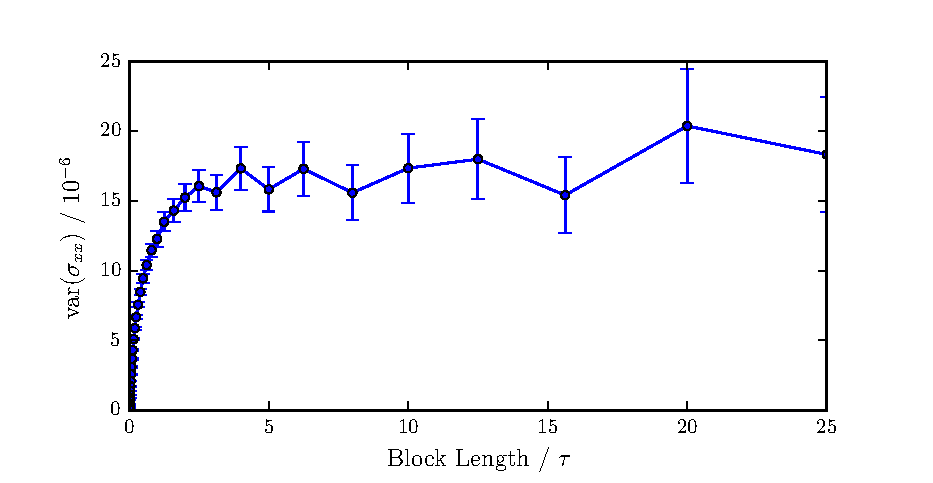
\includegraphics[scale=0.35]{block_average_1e6.eps}
	\caption{The blocking analysis for a simulation time of 10,000,000 timesteps and 1,000,000 timesteps shows clear plateaus in the estimate of the error at block sizes of 10,000 and 5,000 respectively.
This can be used to estimate the size of blocking needed to decorrelate data in the correspinding molecular dynamics simulations.}
\label{blocking}
\end{figure*}

Using a standard binary mixture simulation identical to those used to calculate the Marangoni forces at the interface, a blocking analysis was carried out for a simulation time of $10^{6}$ timesteps and $10^{7}$ timesteps as shown in Fig \ref{blocking}.
These data show a clear plateau at a block size of 10,000 timesteps for the longer simulation time and 5,000 timesteps for the shorter run, with little increase in the error of $\sigma^{2}$ until a much larger block size.
This information can be used to infer a suitable size for block averaging data within a LAMMPS simulation in order to yield sufficient decorrelation of individual samples and a good estimate of the statistical error. 


\subsection{Software details}
All molecular dynamics simulations were carried out using the LAMMPS (Large Atomic and Molecular Massively Parallel Simulator) package.\cite{LAMMPS}
Additional processing was carried out using Numpy.\cite{NumPy}
All graphical figures were plotted using Matplotlib.\cite{MatPlotLib}

